
% This LaTeX was auto-generated from MATLAB code.
% To make changes, update the MATLAB code and republish this document.

\documentclass{article}
\usepackage{graphicx}
\usepackage{color}

\sloppy
\definecolor{lightgray}{gray}{0.5}
\setlength{\parindent}{0pt}

\begin{document}

    
    \begin{verbatim}
G_CL  = tf([5 0 0],[-25 40 2000 0 0]);
C2tf = tf(C);
Cr = C2tf(1);
Cy = C2tf(2);
T  = Cr*feedback(G_CL,Cy,1);
step(T);
grid on;
C
\end{verbatim}

        \color{lightgray} \begin{verbatim}
C =
 
                       1                s    
  u = Kp (b*r-y) + Ki --- (r-y) + Kd -------- (c*r-y)
                       s              Tf*s+1 

  with Kp = -8.89e+03, Ki = -3.82e+04, Kd = -502, Tf = 0.0018, b = 0.89, c = 0.747
 
Continuous-time 2-DOF PIDF controller in parallel form.

\end{verbatim} \color{black}
    
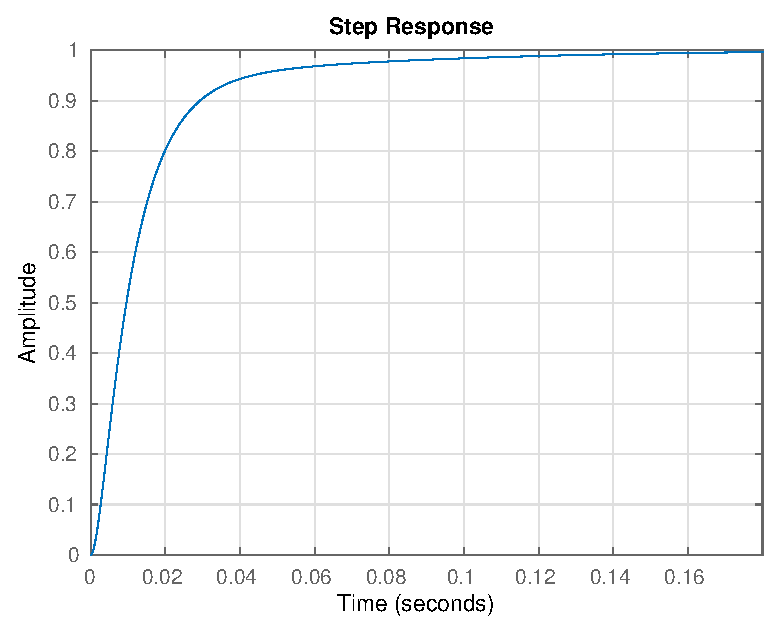
\includegraphics [width=4in]{pr3_01.eps}



\end{document}
    
